\section{Experimental design}
The protocol was committed before any new score was computed (\texttt{91619f1}) on frozen main \texttt{244a9bf}, and settings stay fixed after scoring. The research questions cover structural frequency (RQ1), evidence complementarity (RQ2), coverage and redundancy (RQ3), repair (RQ4), utility (RQ5) and stability and uncertainty (RQ6).
\begin{table}[!t]
\centering
\caption{Frozen task datasets and literal positive counts.}\label{tab:datasets}
\footnotesize\setlength{\tabcolsep}{3pt}
\begin{tabular}{lrrrrrr}
\toprule
Dataset & Rows & TRAIN & TEST & TRAIN+ & TEST+ & Candidates \\
\midrule
Abalone19 & 4174 & 3340 & 834 & 26 & 6 & 200 \\
Ecoli4 & 336 & 269 & 67 & 16 & 4 & 201 \\
page-blocks0 & 5472 & 4377 & 1095 & 447 & 112 & 200 \\
\bottomrule
\end{tabular}
\end{table}


\begin{figure}[!t]\centering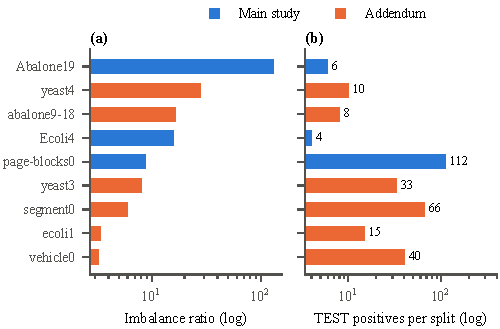
\includegraphics[width=\linewidth]{figures/datasets.pdf}
\caption{Datasets of the main study and the exploratory addendum (Section~\ref{sec:addendum}). (a) Imbalance ratio. (b) TEST positives per fresh split, which bound inference on the smallest datasets.}\label{fig:datasets}\end{figure}

\textit{Track A (historical fixed split).} Datasets, original TRAIN/TEST identities and the 601 candidates are unchanged; candidates depended on original TRAIN and are never reassigned, the previously evaluated TEST set is reused descriptively, and exact TRAIN/TEST feature overlap is recorded. Budgets of 56, 70 and 49 for Abalone19, Ecoli4 and page-blocks0 are inherited. Raw-labeled random keeps evaluable integer defects but excludes absent labels and unsupported features, schema random requires full compliance, and admitted random draws from the combined-admitted pool shared by the four deterministic selectors; random controls use seeds $13,29,43,61,79$. Admission ablations apply the same quality-coverage selector after structure-only, local, global or combined eligibility, so pool size is part of the intervention. All 138 historical utility comparisons are replayed from saved predictions; B1/B2/B3 stay frozen and are intersected with structural completeness. The archived raw scorer could read a missing class as the string \texttt{nan}, so those scores are not used as complete binary-record comparisons. External comparators append exactly $b$ minority rows with ROS or SMOTE (SMOTENC for categorical Abalone19), with TRAIN-fitted standardization and unrounded page-blocks0 integers, and balanced logistic loss is a non-generative comparator. These are training alternatives, not same-pool curation; mixed-class historical subsets may add fewer than $b$ minority rows in hybrid regimes.

\textit{Track B (fresh offline splits).} Five deterministic stratified 80/20 splits per dataset use the same seeds, and every split refits preprocessing, generation, evidence and geometry on its own TRAIN. Pools hold $4b$ minority records from SMOTENC (Abalone19), SMOTE (Ecoli4) or ROS (integer-declared page-blocks0, which adds no new support), with $k=\min(5,n_+-1)$. Six curators (schema random, admitted random, source order, farthest-first, coverage-greedy, quality-coverage) are compared with real-only, class-weighted and ROS/SMOTE training. Minority-only pools allow hybrid augmentation but not pure TSTR. This tests offline curation, not LLM candidate quality, and because holdouts overlap, across-split SD describes variability, not an independent-sample standard error.

\textit{Classifiers, metrics and uncertainty.} Logistic regression (liblinear, at most 300 iterations) and random forest (50 trees) use seed 42, with imputation, scaling and encoding fitted only on the training population. TRTR trains on real TRAIN, pure TSTR on synthetic rows and hybrid on real TRAIN plus synthetic positives. We report $F_1=2TP/(2TP+FP+FN)$, balanced accuracy, MCC, AP (the step integral $\sum_k(R_k-R_{k-1})P_k$, not trapezoidal area) and AUROC; point MCC uses the frozen zero convention for degenerate margins, and undefined cases are counted explicitly. Historical intervals use 2,000 stratified paired resamples of saved predictions (seed 20261025, 95\% percentile bounds), resampling positive and negative indices within strata identically across paired methods. Primary pairs compare original quality-coverage with schema and admitted random (seed 13), hybrid quality-coverage with TRTR, and repaired with original quality-coverage. Intervals condition on fitted models and observed TEST, excluding generation and refitting uncertainty. No multiplicity-adjusted significance claim is made.
